% Options for packages loaded elsewhere
% Options for packages loaded elsewhere
\PassOptionsToPackage{unicode}{hyperref}
\PassOptionsToPackage{hyphens}{url}
%
\documentclass[
  14pt,
  ignorenonframetext,
  aspectratio=169,
]{beamer}
\newif\ifbibliography
\usepackage{pgfpages}
\setbeamertemplate{caption}[numbered]
\setbeamertemplate{caption label separator}{: }
\setbeamercolor{caption name}{fg=normal text.fg}
\beamertemplatenavigationsymbolsempty
% remove section numbering
\setbeamertemplate{part page}{
  \centering
  \begin{beamercolorbox}[sep=16pt,center]{part title}
    \usebeamerfont{part title}\insertpart\par
  \end{beamercolorbox}
}
\setbeamertemplate{section page}{
  \centering
  \begin{beamercolorbox}[sep=12pt,center]{section title}
    \usebeamerfont{section title}\insertsection\par
  \end{beamercolorbox}
}
\setbeamertemplate{subsection page}{
  \centering
  \begin{beamercolorbox}[sep=8pt,center]{subsection title}
    \usebeamerfont{subsection title}\insertsubsection\par
  \end{beamercolorbox}
}
% Prevent slide breaks in the middle of a paragraph
\widowpenalties 1 10000
\raggedbottom
\usepackage{iftex}
\ifPDFTeX
  \usepackage[T1]{fontenc}
  \usepackage[utf8]{inputenc}
  \usepackage{textcomp} % provide euro and other symbols
\else % if luatex or xetex
  \usepackage{unicode-math} % this also loads fontspec
  \defaultfontfeatures{Scale=MatchLowercase}
  \defaultfontfeatures[\rmfamily]{Ligatures=TeX,Scale=1}
\fi
\usepackage{lmodern}

\usetheme[]{monash}
\ifPDFTeX\else
  % xetex/luatex font selection
\fi
% Use upquote if available, for straight quotes in verbatim environments
\IfFileExists{upquote.sty}{\usepackage{upquote}}{}
\IfFileExists{microtype.sty}{% use microtype if available
  \usepackage[]{microtype}
  \UseMicrotypeSet[protrusion]{basicmath} % disable protrusion for tt fonts
}{}
\makeatletter
\@ifundefined{KOMAClassName}{% if non-KOMA class
  \IfFileExists{parskip.sty}{%
    \usepackage{parskip}
  }{% else
    \setlength{\parindent}{0pt}
    \setlength{\parskip}{6pt plus 2pt minus 1pt}}
}{% if KOMA class
  \KOMAoptions{parskip=half}}
\makeatother

\usepackage{color}
\usepackage{fancyvrb}
\newcommand{\VerbBar}{|}
\newcommand{\VERB}{\Verb[commandchars=\\\{\}]}
\DefineVerbatimEnvironment{Highlighting}{Verbatim}{commandchars=\\\{\}}
% Add ',fontsize=\small' for more characters per line
\usepackage{framed}
\definecolor{shadecolor}{RGB}{248,248,248}
\newenvironment{Shaded}{\begin{snugshade}}{\end{snugshade}}
\newcommand{\AlertTok}[1]{\textcolor[rgb]{0.94,0.16,0.16}{#1}}
\newcommand{\AnnotationTok}[1]{\textcolor[rgb]{0.56,0.35,0.01}{\textbf{\textit{#1}}}}
\newcommand{\AttributeTok}[1]{\textcolor[rgb]{0.13,0.29,0.53}{#1}}
\newcommand{\BaseNTok}[1]{\textcolor[rgb]{0.00,0.00,0.81}{#1}}
\newcommand{\BuiltInTok}[1]{#1}
\newcommand{\CharTok}[1]{\textcolor[rgb]{0.31,0.60,0.02}{#1}}
\newcommand{\CommentTok}[1]{\textcolor[rgb]{0.56,0.35,0.01}{\textit{#1}}}
\newcommand{\CommentVarTok}[1]{\textcolor[rgb]{0.56,0.35,0.01}{\textbf{\textit{#1}}}}
\newcommand{\ConstantTok}[1]{\textcolor[rgb]{0.56,0.35,0.01}{#1}}
\newcommand{\ControlFlowTok}[1]{\textcolor[rgb]{0.13,0.29,0.53}{\textbf{#1}}}
\newcommand{\DataTypeTok}[1]{\textcolor[rgb]{0.13,0.29,0.53}{#1}}
\newcommand{\DecValTok}[1]{\textcolor[rgb]{0.00,0.00,0.81}{#1}}
\newcommand{\DocumentationTok}[1]{\textcolor[rgb]{0.56,0.35,0.01}{\textbf{\textit{#1}}}}
\newcommand{\ErrorTok}[1]{\textcolor[rgb]{0.64,0.00,0.00}{\textbf{#1}}}
\newcommand{\ExtensionTok}[1]{#1}
\newcommand{\FloatTok}[1]{\textcolor[rgb]{0.00,0.00,0.81}{#1}}
\newcommand{\FunctionTok}[1]{\textcolor[rgb]{0.13,0.29,0.53}{\textbf{#1}}}
\newcommand{\ImportTok}[1]{#1}
\newcommand{\InformationTok}[1]{\textcolor[rgb]{0.56,0.35,0.01}{\textbf{\textit{#1}}}}
\newcommand{\KeywordTok}[1]{\textcolor[rgb]{0.13,0.29,0.53}{\textbf{#1}}}
\newcommand{\NormalTok}[1]{#1}
\newcommand{\OperatorTok}[1]{\textcolor[rgb]{0.81,0.36,0.00}{\textbf{#1}}}
\newcommand{\OtherTok}[1]{\textcolor[rgb]{0.56,0.35,0.01}{#1}}
\newcommand{\PreprocessorTok}[1]{\textcolor[rgb]{0.56,0.35,0.01}{\textit{#1}}}
\newcommand{\RegionMarkerTok}[1]{#1}
\newcommand{\SpecialCharTok}[1]{\textcolor[rgb]{0.81,0.36,0.00}{\textbf{#1}}}
\newcommand{\SpecialStringTok}[1]{\textcolor[rgb]{0.31,0.60,0.02}{#1}}
\newcommand{\StringTok}[1]{\textcolor[rgb]{0.31,0.60,0.02}{#1}}
\newcommand{\VariableTok}[1]{\textcolor[rgb]{0.00,0.00,0.00}{#1}}
\newcommand{\VerbatimStringTok}[1]{\textcolor[rgb]{0.31,0.60,0.02}{#1}}
\newcommand{\WarningTok}[1]{\textcolor[rgb]{0.56,0.35,0.01}{\textbf{\textit{#1}}}}

\usepackage{longtable,booktabs,array}
\newcounter{none} % for unnumbered tables
\usepackage{calc} % for calculating minipage widths
\usepackage{caption}
% Make caption package work with longtable
\makeatletter
\def\fnum@table{\tablename~\thetable}
\makeatother
\usepackage{graphicx}
\makeatletter
\newsavebox\pandoc@box
\newcommand*\pandocbounded[1]{% scales image to fit in text height/width
  \sbox\pandoc@box{#1}%
  \Gscale@div\@tempa{\textheight}{\dimexpr\ht\pandoc@box+\dp\pandoc@box\relax}%
  \Gscale@div\@tempb{\linewidth}{\wd\pandoc@box}%
  \ifdim\@tempb\p@<\@tempa\p@\let\@tempa\@tempb\fi% select the smaller of both
  \ifdim\@tempa\p@<\p@\scalebox{\@tempa}{\usebox\pandoc@box}%
  \else\usebox{\pandoc@box}%
  \fi%
}
% Set default figure placement to htbp
\def\fps@figure{htbp}
\makeatother





\setlength{\emergencystretch}{3em} % prevent overfull lines

\providecommand{\tightlist}{%
  \setlength{\itemsep}{0pt}\setlength{\parskip}{0pt}}



 


% Colors
\definecolor{shadecolor}{RGB}{225,225,225}
\setbeamercolor{description item}{fg=Orange}
\definecolor{MonashBlue}{RGB}{66,109,152}
\definecolor{burntorange}{rgb}{0.8, 0.33, 0.0}

% Packages
\usepackage{amsmath, bm, amssymb, amsthm, mathrsfs,pifont}
\usepackage{url}
\usepackage{multirow, booktabs, float, textcmds, siunitx}
\usepackage{bm,booktabs,animate,ragged2e,multicol,microtype,hyperref}
\usepackage{fontawesome5}

% Figures
\graphicspath{{figs/}}

% Fonts
\fontsize{13}{15}\sf
\setbeamerfont{title}{series=\bfseries,parent=structure,size=\fontsize{24}{24}}
\ifcsname Shaded\endcsname
  \definecolor{shadecolor}{RGB}{225,225,225}
  \renewenvironment{Shaded}{\vspace*{0.15cm}\color{black}\fontsize{10}{10}\sf\begin{snugshade}\color{black}}{\end{snugshade}}
\fi

% gt dependencies
\usepackage{longtable,caption,setspace}
\captionsetup{font={small,stretch=0.80}}

% My definitions

\def\E{\text{E}}
\def\V{\text{Var}}
\def\up#1{\raisebox{-0.3cm}{#1}}
\def\pred#1#2#3{\hat{#1}_{#2|#3}}
\def\damped{$_\text{d}$}
\def\h+{h_{m}^{+}}
\def\str#1{\rlap{#1}\textcolor{red}{\rule{1cm}{0.1cm}}}

\def\st#1{\rlap{#1}\textcolor{red}{\rule{1cm}{0.1cm}}}
\def\bY{\bm{y}}
\def\by{\bm{y}}
\def\bS{\bm{S}}
\def\bI{\text{\rm\textbf{I}}}
\def\bbeta{\bm{\beta}}
\def\bSigma{\bm{\Sigma}}
\def\bW{\bm{\Sigma}}
\def\Var{\text{Var}}
\def\var{\text{Var}}
\def\bOmega{\bm{\Omega}}
\def\bLambda{\bm{\Lambda}}
\let\mc\multicolumn
\def\hl{\color[RGB]{230, 172, 0}}

\def\forecast{\begin{alertblock}{}\fontsize{10}{11}\sf
 A forecast is an estimate of the probability distribution of a variable to be observed in the future.
\end{alertblock}}

\def\simfutures{\begin{textblock}{2.9}(12.8,7.7)
\begin{block}{}\fontsize{10}{11}\sf
Simulated futures from an ETS model
\end{block}\end{textblock}}

\setbeamertemplate{title page}
{\placefig{0}{-0.5}{width=1.01\paperwidth,height=1.45\paperheight}{africa1.jpg}
\begin{textblock}{8.5}(.5,0.2)
  \raggedright\fontsize{20}{20}\selectfont\bfseries\sffamily\textcolor{white}{\inserttitle}\\[0.2cm]
  \fontsize{12}{12}\selectfont\bfseries\sffamily\textcolor{white}{\insertsubtitle}
  \end{textblock}
\placefig{.5}{6.2}{width=2.4cm}{tsibble.png}
\placefig{2.9}{6.2}{width=2.4cm}{feasts.png}
\placefig{5.3}{6.2}{width=2.4cm}{fable.png}
\begin{textblock}{7.5}(10.6,-.1)
  {\fontsize{9}{9}\sf\color{white}https://workshop.f4sg.org/africast/}
\end{textblock}
}

% Tikz plots
\usepackage{tikz}
\usetikzlibrary{trees,shapes,arrows,matrix,shadows,positioning,calc}
\tikzstyle{decision} = [diamond, draw, fill=blue!20,
    text width=4.5em, text badly centered, node distance=4cm, inner sep=0pt]
\tikzstyle{block} = [rectangle, draw, fill=blue!20,
    text width=5cm, text centered, rounded corners, minimum height=4em]
\tikzstyle{line} = [draw, thick, -latex']
\tikzstyle{cloud} = [draw, ellipse,fill=red!20, node distance=3cm,
    minimum height=2em, text centered]
\tikzstyle{connector} = [->,thick]

\tikzset{
  basic/.style  = {draw, text width=2cm, font=\sffamily, rectangle},
  root/.style   = {basic, text width=3cm, rounded corners=2pt, thin, align=center, fill=red!30},
  level 2a/.style = {basic, rounded corners=2pt, thin,align=center, fill=blue!50, text width=7em},
  level 2b/.style = {basic, rounded corners=2pt, thin,align=center, fill=green!50, text width=7em},
  level 3a/.style = {basic, rounded corners=2pt, thin, align=center, fill=blue!30, text width=4em},
  level 3b/.style = {basic, rounded corners=2pt, thin, align=center, fill=green!30, text width=4em},
  level 4a/.style = {basic, rounded corners=2pt, thin, align=left, fill=blue!10, text width=3.5em},
  level 4b/.style = {basic, rounded corners=2pt, thin, align=left, fill=green!10, text width=3.5em}
}

% % BIBLIOGRAPHIES
% \usepackage[style=authoryear,bibencoding=utf8,minnames=1,maxnames=4, maxbibnames=99,natbib=true,dashed=false,terseinits=true,giveninits=true,uniquename=false,uniquelist=false,labeldate=true,doi=false, isbn=false, natbib=true,backend=biber]{biblatex}

% \DeclareFieldFormat{url}{\url{#1}}
% \DeclareFieldFormat[article]{pages}{#1}
% \DeclareFieldFormat[inproceedings]{pages}{\lowercase{pp.}#1}
% \DeclareFieldFormat[incollection]{pages}{\lowercase{pp.}#1}
% \DeclareFieldFormat[article]{volume}{\mkbibbold{#1}}
% \DeclareFieldFormat[article]{number}{\mkbibparens{#1}}
% \DeclareFieldFormat[article]{title}{\MakeCapital{#1}}
% \DeclareFieldFormat[article]{url}{}
% \DeclareFieldFormat[Techreport]{Url}{}
% \DeclareFieldFormat[book]{url}{}
% \DeclareFieldFormat[inbook]{url}{}
% \DeclareFieldFormat[incollection]{url}{}
% \DeclareFieldFormat[inproceedings]{url}{}
% \DeclareFieldFormat[inproceedings]{title}{#1}
% \DeclareFieldFormat{shorthandwidth}{#1}
% %\DeclareFieldFormat{extrayear}{}
% % No dot before number of articles
% \usepackage{xpatch}
% \xpatchbibmacro{volume+number+eid}{\setunit*{\adddot}}{}{}{}
% % Remove In: for an article.
% \renewbibmacro{in:}{%
%   \ifentrytype{article}{}{%
%   \printtext{\bibstring{in}\intitlepunct}}}

% \AtEveryBibitem{\clearfield{month}}
% \AtEveryCitekey{\clearfield{month}}
% \AtBeginBibliography{\fontsize{11}{11}\sf}
\setbeamertemplate{frametitle continuation}{}
\makeatletter
\@ifpackageloaded{caption}{}{\usepackage{caption}}
\AtBeginDocument{%
\ifdefined\contentsname
  \renewcommand*\contentsname{Table of contents}
\else
  \newcommand\contentsname{Table of contents}
\fi
\ifdefined\listfigurename
  \renewcommand*\listfigurename{List of Figures}
\else
  \newcommand\listfigurename{List of Figures}
\fi
\ifdefined\listtablename
  \renewcommand*\listtablename{List of Tables}
\else
  \newcommand\listtablename{List of Tables}
\fi
\ifdefined\figurename
  \renewcommand*\figurename{Figure}
\else
  \newcommand\figurename{Figure}
\fi
\ifdefined\tablename
  \renewcommand*\tablename{Table}
\else
  \newcommand\tablename{Table}
\fi
}
\@ifpackageloaded{float}{}{\usepackage{float}}
\floatstyle{ruled}
\@ifundefined{c@chapter}{\newfloat{codelisting}{h}{lop}}{\newfloat{codelisting}{h}{lop}[chapter]}
\floatname{codelisting}{Listing}
\newcommand*\listoflistings{\listof{codelisting}{List of Listings}}
\makeatother
\makeatletter
\makeatother
\makeatletter
\@ifpackageloaded{caption}{}{\usepackage{caption}}
\@ifpackageloaded{subcaption}{}{\usepackage{subcaption}}
\makeatother

\usepackage{bookmark}
\IfFileExists{xurl.sty}{\usepackage{xurl}}{} % add URL line breaks if available
\urlstyle{same}
% fallback for those not using the hyperref driver hyperxmp:
\makeatletter
\@ifundefined{xmpquote}{\newcommand{\xmpquote}[1]{#1}}{}
\makeatother
\hypersetup{
  pdftitle={Africast-Time Series Analysis \& Forecasting Using R},
  hidelinks,
  pdfcreator={LaTeX via pandoc}}


\title{\texorpdfstring{Africast-Time Series Analysis \& Forecasting
Using R}{Africast-Time Series Analysis \& Forecasting Using R}}
\subtitle{\texorpdfstring{6. Forecasting with regression, how to
represent temporal structure with
regressors}{6. Forecasting with regression, how to represent temporal structure with regressors}}
\author{}
\date{27 November 2025}

\begin{document}
\frame{\titlepage}


\begin{frame}{Outline}
\protect\phantomsection\label{outline}
\vspace*{0.7cm}\tableofcontents
\end{frame}

\section{The linear model with time
series}\label{the-linear-model-with-time-series}

\begin{frame}{Regression models}
\protect\phantomsection\label{regression-models}
\begin{itemize}
\tightlist
\item
  To \textbf{explain}
\item
  To \textbf{forecast}
\end{itemize}

\vspace*{0.3cm}

\begin{itemize}
\tightlist
\item
  Simple linear regression model(SLR)
\item
  Multiple linear regression model (MLR)
\end{itemize}
\end{frame}

\begin{frame}[fragile]{SLR model in thoery}
\protect\phantomsection\label{slr-model-in-thoery}
Regression model allows for a linear relationship between the forecast
variable \(y\) and a single predictor variable \(x\).

\fontsize{13}{15}\sf

\begin{block}{}\vspace*{-0.3cm}
$$
  y_t = \beta_0 + \beta_1 x_{t} + \varepsilon_t.
$$
\end{block}

\begin{itemize}
\tightlist
\item
  \(y_t\) is the variable we want to predict: the \texttt{response}
  variable
\item
  Each \(x_{t}\) is numerical and is called a \texttt{predictor}
\item
  \(\beta_0\) and \(\beta_1\) are regression coefficients
\end{itemize}
\end{frame}

\begin{frame}[fragile]{SLR model in practice}
\protect\phantomsection\label{slr-model-in-practice}
\fontsize{13}{15}\sf

In practice, of course, we have a collection of observations but we do
not know the values of the coefficients \(\hat\beta_0\),
\(\hat\beta_1\). These need to be estimated from the data.

\begin{block}{}\vspace*{-0.3cm}
$$
  y_t = \hat\beta_0 + \hat\beta_1 x_{t}.
$$
\end{block}

\begin{itemize}
\tightlist
\item
  \(y_t\) is the \texttt{response} variable
\item
  Each \(x_{t}\) is a \texttt{predictor}
\item
  \(\hat\beta_0\) is the estimated intercept
\item
  \(\hat\beta_1\) is the estimated slope
\end{itemize}
\end{frame}

\begin{frame}{What is the best fit}
\protect\phantomsection\label{what-is-the-best-fit}
\fontsize{11}{13}\sf

\begin{itemize}
\tightlist
\item
  There are many ways that a straight line can be laid on the scatter
\item
  Best known criterion is called Ordinary Least Squares(OLS)
\end{itemize}

\begin{center}
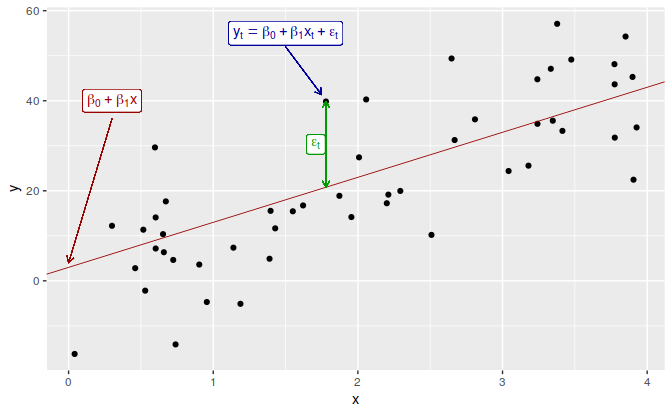
\includegraphics[width=0.7\linewidth,height=\textheight,keepaspectratio]{figs/SLRpop1-1.png}
\end{center}
\end{frame}

\begin{frame}{Estimation of the model}
\protect\phantomsection\label{estimation-of-the-model}
That is, we find the values of \(\beta_0\) and \(\beta_1\) which
minimize

\begin{block}{}\vspace*{-0.3cm}
$$
  \sum_{i=1}^N e_{i}^2 = \sum_{i=1}^N (y_{i} - \beta_{0} - \beta_{1}x_{i})^2. 
$$
\end{block}

\begin{itemize}
\tightlist
\item
  This is called \emph{least squares} estimation because it gives the
  least value of the sum of squared errors.
\item
  Finding the best estimates of the coefficients is often called
  \emph{fitting} the model to the data.
\item
  We refer to the \emph{estimated} coefficients using the notation
  \(\hat\beta_{0},\hat\beta_{1}\).
\end{itemize}
\end{frame}

\begin{frame}[fragile]{Example: US consumption expenditure}
\protect\phantomsection\label{example-us-consumption-expenditure}
\fontsize{11}{13}\sf

\begin{Shaded}
\begin{Highlighting}[]
\NormalTok{us\_change }\SpecialCharTok{\%\textgreater{}\%}
  \FunctionTok{gather}\NormalTok{(}\StringTok{"Measure"}\NormalTok{, }\StringTok{"Change"}\NormalTok{, Consumption, Income) }\SpecialCharTok{\%\textgreater{}\%}
  \FunctionTok{autoplot}\NormalTok{(Change) }\SpecialCharTok{+}
  \FunctionTok{ylab}\NormalTok{(}\StringTok{"\% change"}\NormalTok{) }\SpecialCharTok{+} \FunctionTok{xlab}\NormalTok{(}\StringTok{"Year"}\NormalTok{)}
\end{Highlighting}
\end{Shaded}

\pandocbounded{\includegraphics[keepaspectratio]{03_regression_files/figure-beamer/ConsInc-1.pdf}}
\end{frame}

\begin{frame}{Example: US consumption expenditure}
\protect\phantomsection\label{example-us-consumption-expenditure-1}
\pandocbounded{\includegraphics[keepaspectratio]{03_regression_files/figure-beamer/ConsInc2-1.pdf}}
\end{frame}

\begin{frame}[fragile]{Example: US consumption expenditure}
\protect\phantomsection\label{example-us-consumption-expenditure-2}
\fontsize{9}{9}\sf

\begin{Shaded}
\begin{Highlighting}[]
\NormalTok{fit\_cons }\OtherTok{\textless{}{-}}\NormalTok{ us\_change }\SpecialCharTok{\%\textgreater{}\%}
  \FunctionTok{model}\NormalTok{(}\AttributeTok{lm =} \FunctionTok{TSLM}\NormalTok{(Consumption }\SpecialCharTok{\textasciitilde{}}\NormalTok{ Income))}
\FunctionTok{report}\NormalTok{(fit\_cons)}
\end{Highlighting}
\end{Shaded}

\begin{verbatim}
Series: Consumption 
Model: TSLM 

Residuals:
   Min     1Q Median     3Q    Max 
-2.408 -0.318  0.026  0.300  1.452 

Coefficients:
            Estimate Std. Error t value Pr(>|t|)    
(Intercept)   0.5451     0.0557    9.79  < 2e-16 ***
Income        0.2806     0.0474    5.91  1.6e-08 ***
---
Signif. codes:  0 '***' 0.001 '**' 0.01 '*' 0.05 '.' 0.1 ' ' 1

Residual standard error: 0.603 on 185 degrees of freedom
Multiple R-squared: 0.159,  Adjusted R-squared: 0.154
F-statistic:   35 on 1 and 185 DF, p-value: 2e-08
\end{verbatim}
\end{frame}

\begin{frame}{Multiple regression}
\protect\phantomsection\label{multiple-regression}
\begin{itemize}
\tightlist
\item
  In multiple regression there is one variable to be forecast and
  several predictor variables.
\item
  The basic concept is that we forecast the time series of interest
  \(y\) assuming that it has a linear relationship with other time
  series \(x_1\), \(x_2\), \ldots., \(x_K\)
\item
  We might forecast daily A\&E attendance \(y\) using temperature
  \(x_1\) and GP visits \(x_2\) as predictors.
\end{itemize}
\end{frame}

\begin{frame}{How many variable can we add?}
\protect\phantomsection\label{how-many-variable-can-we-add}
You can add as many as you want but be aware of:

\begin{itemize}
\tightlist
\item
  Over-fitting
\item
  Multicollinearity
\end{itemize}
\end{frame}

\begin{frame}[fragile]{Multiple regression and forecasting}
\protect\phantomsection\label{multiple-regression-and-forecasting}
\fontsize{13}{15}\sf

\begin{block}{}\vspace*{-0.3cm}
$$
  y_t = \beta_0 + \beta_1 x_{1,t} + \beta_2 x_{2,t} + \cdots + \beta_kx_{k,t} + \varepsilon_t.
$$

\end{block}

\begin{itemize}
\item
  \(y_t\) is the variable we want to predict: the \texttt{response}
  variable
\item
  Each \(x_{j,t}\) is numerical and is called a \texttt{predictor}. They
  are usually assumed to be known for all past and future times.
\item
  The coefficients \(\beta_1,\dots,\beta_k\) measure the effect of each
  predictor after taking account of the effect of all other predictors
  in the model.
\end{itemize}

That is, the coefficients measure the \textbf{marginal effects}.

\begin{itemize}
\tightlist
\item
  \(\varepsilon_t\) is a white noise error term
\end{itemize}
\end{frame}

\begin{frame}{Estimation of the model}
\protect\phantomsection\label{estimation-of-the-model-1}
We find the values of \(\hat\beta_{0},\dots,\hat\beta_{k}\) which
minimize

\[ 
\sum_{i=1}^N e_{i}^2 = \sum_{i=1}^N (y_{i} - \beta_{0} - \beta_{1}x_{1,i} - \cdots - \beta_{k} x_{k,i})^2. 
\]

\begin{itemize}
\tightlist
\item
  This is called \emph{least squares} estimation because it gives the
  least value of the sum of squared errors
\item
  Finding the best estimates of the coefficients is often called
  \emph{fitting} the model to the data
\item
  We refer to the \emph{estimated} coefficients using the notation
  \(\hat\beta_{0},\dots,\hat\beta_{k}\).
\end{itemize}
\end{frame}

\begin{frame}[fragile]{Useful predictors in linear regression}
\protect\phantomsection\label{useful-predictors-in-linear-regression}
\textbf{Linear trend} \[
  x_t = t
\]

\begin{itemize}
\tightlist
\item
  \(t=1,2,\dots,T\)
\item
  Strong assumption that trend will continue.
\item
  use special function \texttt{trend()}
\end{itemize}

\textbf{Seasonality}

\begin{itemize}
\tightlist
\item
  Seasonality will be considered based on the interval of index
\item
  use special function \texttt{season()}
\end{itemize}
\end{frame}

\begin{frame}{Example: US consumption expenditure}
\protect\phantomsection\label{example-us-consumption-expenditure-3}
\pandocbounded{\includegraphics[keepaspectratio]{03_regression_files/figure-beamer/MultiPredictors-1.pdf}}
\end{frame}

\begin{frame}{Example: US consumption expenditure}
\protect\phantomsection\label{example-us-consumption-expenditure-4}
\pandocbounded{\includegraphics[keepaspectratio]{03_regression_files/figure-beamer/ScatterMatrix-1.pdf}}
\end{frame}

\begin{frame}[fragile]{Example: US consumption expenditure}
\protect\phantomsection\label{example-us-consumption-expenditure-5}
\fontsize{7.4}{7.4}\sf

\begin{Shaded}
\begin{Highlighting}[]
\NormalTok{fit\_consMR }\OtherTok{\textless{}{-}}\NormalTok{ us\_change }\SpecialCharTok{\%\textgreater{}\%}
  \FunctionTok{model}\NormalTok{(}\AttributeTok{lm =} \FunctionTok{TSLM}\NormalTok{(Consumption }\SpecialCharTok{\textasciitilde{}}\NormalTok{ Income }\SpecialCharTok{+}\NormalTok{ Production }\SpecialCharTok{+}\NormalTok{ Unemployment }\SpecialCharTok{+}\NormalTok{ Savings))}
\FunctionTok{report}\NormalTok{(fit\_consMR)}
\end{Highlighting}
\end{Shaded}

\begin{verbatim}
Series: Consumption 
Model: TSLM 

Residuals:
   Min     1Q Median     3Q    Max 
-0.883 -0.176 -0.037  0.153  1.206 

Coefficients:
             Estimate Std. Error t value Pr(>|t|)    
(Intercept)   0.26729    0.03721    7.18  1.7e-11 ***
Income        0.71448    0.04219   16.93  < 2e-16 ***
Production    0.04589    0.02588    1.77    0.078 .  
Unemployment -0.20477    0.10550   -1.94    0.054 .  
Savings      -0.04527    0.00278  -16.29  < 2e-16 ***
---
Signif. codes:  0 '***' 0.001 '**' 0.01 '*' 0.05 '.' 0.1 ' ' 1

Residual standard error: 0.329 on 182 degrees of freedom
Multiple R-squared: 0.754,  Adjusted R-squared: 0.749
F-statistic:  139 on 4 and 182 DF, p-value: <2e-16
\end{verbatim}
\end{frame}

\begin{frame}{Example: US consumption expenditure}
\protect\phantomsection\label{example-us-consumption-expenditure-6}
\pandocbounded{\includegraphics[keepaspectratio]{03_regression_files/figure-beamer/usfitted1-1.pdf}}
\end{frame}

\begin{frame}{Example: US consumption expenditure}
\protect\phantomsection\label{example-us-consumption-expenditure-7}
\pandocbounded{\includegraphics[keepaspectratio]{03_regression_files/figure-beamer/usfitted2-1.pdf}}
\end{frame}

\begin{frame}[fragile]{Example: US consumption expenditure}
\protect\phantomsection\label{example-us-consumption-expenditure-8}
\begin{Shaded}
\begin{Highlighting}[]
\FunctionTok{augment}\NormalTok{(fit\_consMR) }\SpecialCharTok{\%\textgreater{}\%}
  \FunctionTok{gg\_tsdisplay}\NormalTok{(.resid, }\AttributeTok{plot\_type=}\StringTok{"hist"}\NormalTok{)}
\end{Highlighting}
\end{Shaded}

\pandocbounded{\includegraphics[keepaspectratio]{03_regression_files/figure-beamer/unnamed-chunk-2-1.pdf}}
\end{frame}

\section{Evaluating the regression
model}\label{evaluating-the-regression-model}

\begin{frame}{Multiple regression and forecasting}
\protect\phantomsection\label{multiple-regression-and-forecasting-1}
For forecasting purposes, we require the following assumptions:

\begin{itemize}
\item
  \(\varepsilon_t\) are uncorrelated and zero mean
\item
  \(\varepsilon_t\) are uncorrelated with each \(x_{j,t}\). \pause
\end{itemize}

It is \textbf{useful} to also have
\(\varepsilon_t \sim \text{N}(0,\sigma^2)\) when producing prediction
intervals or doing statistical tests.
\end{frame}

\begin{frame}[fragile]{Residual diagnostics}
\protect\phantomsection\label{residual-diagnostics}
There are a series of plots that should be produced in order to check
different aspects of the fitted model and the underlying assumptions.

\begin{enumerate}
\tightlist
\item
  check if residuals are uncorrelated using \texttt{ACF}
\item
  Check if residuals are normally distributed
\end{enumerate}
\end{frame}

\begin{frame}{Residual scatterplots}
\protect\phantomsection\label{residual-scatterplots}
Useful for spotting outliers and whether the linear model was
appropriate.

\begin{itemize}
\item
  Scatterplot of residuals \(\varepsilon_t\) against each predictor
  \(x_{j,t}\).
\item
  Scatterplot residuals against the fitted values \(\hat y_t\)
\item
  Expect to see scatterplots resembling a horizontal band with no values
  too far from the band and no patterns such as curvature or increasing
  spread.
\end{itemize}
\end{frame}

\begin{frame}[fragile]{Example: US consumption expenditure}
\protect\phantomsection\label{example-us-consumption-expenditure-9}
\begin{Shaded}
\begin{Highlighting}[]
\NormalTok{df }\OtherTok{\textless{}{-}} \FunctionTok{left\_join}\NormalTok{(us\_change, }\FunctionTok{residuals}\NormalTok{(fit\_consMR), }\AttributeTok{by =} \StringTok{"Time"}\NormalTok{)}
\NormalTok{p1 }\OtherTok{\textless{}{-}} \FunctionTok{ggplot}\NormalTok{(df, }\FunctionTok{aes}\NormalTok{(}\AttributeTok{x=}\NormalTok{Income, }\AttributeTok{y=}\NormalTok{.resid)) }\SpecialCharTok{+}
  \FunctionTok{geom\_point}\NormalTok{() }\SpecialCharTok{+} \FunctionTok{ylab}\NormalTok{(}\StringTok{"Residuals"}\NormalTok{)}
\NormalTok{p2 }\OtherTok{\textless{}{-}} \FunctionTok{ggplot}\NormalTok{(df, }\FunctionTok{aes}\NormalTok{(}\AttributeTok{x=}\NormalTok{Production, }\AttributeTok{y=}\NormalTok{.resid)) }\SpecialCharTok{+}
  \FunctionTok{geom\_point}\NormalTok{() }\SpecialCharTok{+} \FunctionTok{ylab}\NormalTok{(}\StringTok{"Residuals"}\NormalTok{)}
\NormalTok{p3 }\OtherTok{\textless{}{-}} \FunctionTok{ggplot}\NormalTok{(df, }\FunctionTok{aes}\NormalTok{(}\AttributeTok{x=}\NormalTok{Savings, }\AttributeTok{y=}\NormalTok{.resid)) }\SpecialCharTok{+}
  \FunctionTok{geom\_point}\NormalTok{() }\SpecialCharTok{+} \FunctionTok{ylab}\NormalTok{(}\StringTok{"Residuals"}\NormalTok{)}
\NormalTok{p4 }\OtherTok{\textless{}{-}} \FunctionTok{ggplot}\NormalTok{(df, }\FunctionTok{aes}\NormalTok{(}\AttributeTok{x=}\NormalTok{Unemployment, }\AttributeTok{y=}\NormalTok{.resid)) }\SpecialCharTok{+}
  \FunctionTok{geom\_point}\NormalTok{() }\SpecialCharTok{+} \FunctionTok{ylab}\NormalTok{(}\StringTok{"Residuals"}\NormalTok{)}
\NormalTok{(p1 }\SpecialCharTok{|}\NormalTok{ p2) }\SpecialCharTok{/}\NormalTok{ (p3 }\SpecialCharTok{|}\NormalTok{ p4)}
\end{Highlighting}
\end{Shaded}

\pandocbounded{\includegraphics[keepaspectratio]{03_regression_files/figure-beamer/scatterplot-residuals, options-1.pdf}}
\end{frame}

\begin{frame}{Residual patterns}
\protect\phantomsection\label{residual-patterns}
\begin{itemize}
\item
  If a plot of the residuals vs any predictor in the model shows a
  pattern, then the relationship is non-linear.
\item
  If a plot of the residuals vs any predictor \textbf{not} in the model
  shows a pattern, then the predictor should be added to the model.
\item
  If a plot of the residuals vs fitted values shows a pattern, then
  there is heteroscedasticity in the errors. (Could try a
  transformation.)
\end{itemize}
\end{frame}

\section{Selecting predictors}\label{selecting-predictors}

\begin{frame}{Comparing regression models}
\protect\phantomsection\label{comparing-regression-models}
Computer output for regression will always give the \(R^2\) value. This
is a useful summary of the model.

\begin{itemize}
\item
  It is equal to the square of the correlation between \(y\) and
  \(\hat y\).
\item
  It is often called the ``coefficient of determination'\,'.
\item
  It can also be calculated as follows:
  \(R^2 = \frac{\sum(\hat{y}_t - \bar{y})^2}{\sum(y_t-\bar{y})^2}\)
\item
  It is the proportion of variance accounted for (explained) by the
  predictors.
\end{itemize}
\end{frame}

\begin{frame}[fragile]{Comparing regression models}
\protect\phantomsection\label{comparing-regression-models-1}
\fontsize{11}{13}\sf

However \dots

\begin{itemize}
\item
  \(R^2\) does not allow for \texttt{degrees\ of\ freedom}.
\item
  Adding \emph{any} variable tends to increase the value of \(R^2\),
  even if that variable is irrelevant. \pause
\end{itemize}

To overcome this problem, we can use \emph{adjusted \(R^2\)}:

\begin{block}{}
$$
\bar{R}^2 = 1-(1-R^2)\frac{T-1}{T-k-1}
$$
where $k=$ no.\ predictors and $T=$ no.\ observations.
\end{block}

\pause

\begin{alertblock}{Maximizing $\bar{R}^2$ is equivalent to minimizing $\hat\sigma^2$.}
\centerline{$\displaystyle
\hat{\sigma}^2 = \frac{1}{T-k-1}\sum_{t=1}^T \varepsilon_t^2$
}
\end{alertblock}
\end{frame}

\begin{frame}{Cross-validation}
\protect\phantomsection\label{cross-validation}
\begin{enumerate}
\item
  Remove observation \(t\) from the data set, and fit the model using
  the remaining data. Then compute the error for the omitted observation
\item
  Repeat step 1 for \(t=1,...,T\)
\item
  Compute the MSE from errors obtained in 1. We shall call this the CV
\end{enumerate}
\end{frame}

\begin{frame}{Akaike's Information Criterion}
\protect\phantomsection\label{akaikes-information-criterion}
\begin{block}{}
$$
\text{AIC} = -2\log(L) + 2(k+2)
$$
\end{block}

where \(L\) is the likelihood and \(k\) is the number of predictors in
the model.

\begin{itemize}
\tightlist
\item
  This is a \emph{penalized likelihood} approach.
\item
  \emph{Minimizing} the AIC gives the best model for prediction.
\item
  AIC penalizes terms more heavily than \(\bar{R}^2\).
\item
  Minimizing the AIC is asymptotically equivalent to minimizing MSE via
  leave-one-out cross-validation.
\end{itemize}
\end{frame}

\begin{frame}{Corrected AIC}
\protect\phantomsection\label{corrected-aic}
For small values of \(T\), the AIC tends to select too many predictors,
and so a bias-corrected version of the AIC has been developed.

\begin{block}{}
$$
\text{AIC}_{\text{C}} = \text{AIC} + \frac{2(k+2)(k+3)}{T-k-3}
$$
\end{block}

As with the AIC, the AIC\(_{\text{C}}\) should be minimized.
\end{frame}

\begin{frame}[fragile]{Comparing regression models}
\protect\phantomsection\label{comparing-regression-models-2}
\fontsize{12}{14}\sf

\begin{Shaded}
\begin{Highlighting}[]
\FunctionTok{glance}\NormalTok{(fit\_consMR) }\SpecialCharTok{\%\textgreater{}\%}
  \FunctionTok{select}\NormalTok{(r\_squared, adj\_r\_squared, AIC, AICc, CV)}
\end{Highlighting}
\end{Shaded}

\begin{verbatim}
# A tibble: 1 x 5
  r_squared adj_r_squared   AIC  AICc    CV
      <dbl>         <dbl> <dbl> <dbl> <dbl>
1     0.754         0.749 -409. -409. 0.116
\end{verbatim}
\end{frame}

\begin{frame}{Choosing regression variables}
\protect\phantomsection\label{choosing-regression-variables}
\textbf{Best subsets regression}

\begin{itemize}
\item
  Fit all possible regression models using one or more of the
  predictors.
\item
  Choose the best model based on one of the measures of predictive
  ability (CV, AIC, AICc).
\end{itemize}
\end{frame}

\begin{frame}{Choosing regression variables}
\protect\phantomsection\label{choosing-regression-variables-1}
\textbf{Backwards stepwise regression}

\begin{itemize}
\tightlist
\item
  Start with a model containing all variables.
\item
  Try subtracting one variable at a time. Keep the model if it has lower
  CV or AICc.
\item
  Iterate until no further improvement.
\item
  You can also do forward stepwise
\end{itemize}
\end{frame}

\section{Forecasting with regression}\label{forecasting-with-regression}

\begin{frame}{Ex-ante versus ex-post forecasts}
\protect\phantomsection\label{ex-ante-versus-ex-post-forecasts}
\begin{itemize}
\tightlist
\item
  \emph{Ex ante forecasts} are made using only information available in
  advance.

  \begin{itemize}
  \tightlist
  \item
    require forecasts of predictors
  \end{itemize}
\item
  \emph{Ex post forecasts} are made using later information on the
  predictors.

  \begin{itemize}
  \tightlist
  \item
    useful for studying behaviour of forecasting models.
  \end{itemize}
\item
  trend, seasonal and calendar variables are all known in advance, so
  these don't need to be forecast.
\end{itemize}
\end{frame}

\begin{frame}{Scenario based forecasting}
\protect\phantomsection\label{scenario-based-forecasting}
\begin{itemize}
\tightlist
\item
  Assumes possible scenarios for the predictor variables
\item
  Prediction intervals for scenario based forecasts do not include the
  uncertainty associated with the future values of the predictor
  variables.
\end{itemize}
\end{frame}

\begin{frame}{Building a predictive regression model}
\protect\phantomsection\label{building-a-predictive-regression-model}
\begin{itemize}
\tightlist
\item
  If getting forecasts of predictors is difficult, you can use lagged
  predictors instead.
\end{itemize}

\begin{block}{}\vspace*{-0.3cm}
$$
  beta_0+\beta_1x_{1,t-h}+\dots+\beta_kx_{k,t-h}+\varepsilon_{t}.
$$
\end{block}

\begin{itemize}
\tightlist
\item
  A different model for each forecast horizon \(h\).
\end{itemize}
\end{frame}

\begin{frame}[fragile]{US Consumption}
\protect\phantomsection\label{us-consumption}
\fontsize{10}{11}\sf

\begin{Shaded}
\begin{Highlighting}[]
\NormalTok{fit\_consBest }\OtherTok{\textless{}{-}}\NormalTok{ us\_change }\SpecialCharTok{\%\textgreater{}\%}
  \FunctionTok{model}\NormalTok{(}
    \FunctionTok{TSLM}\NormalTok{(Consumption }\SpecialCharTok{\textasciitilde{}}\NormalTok{ Income }\SpecialCharTok{+}\NormalTok{ Savings }\SpecialCharTok{+}\NormalTok{ Unemployment)}
\NormalTok{  )}

\NormalTok{down\_future }\OtherTok{\textless{}{-}} \FunctionTok{new\_data}\NormalTok{(us\_change, }\DecValTok{4}\NormalTok{) }\SpecialCharTok{\%\textgreater{}\%}
  \FunctionTok{mutate}\NormalTok{(}\AttributeTok{Income =} \SpecialCharTok{{-}}\DecValTok{1}\NormalTok{, }\AttributeTok{Savings =} \SpecialCharTok{{-}}\FloatTok{0.5}\NormalTok{, }\AttributeTok{Unemployment =} \DecValTok{0}\NormalTok{)}
\NormalTok{fc\_down }\OtherTok{\textless{}{-}} \FunctionTok{forecast}\NormalTok{(fit\_consBest, }\AttributeTok{new\_data =}\NormalTok{ down\_future)}

\NormalTok{up\_future }\OtherTok{\textless{}{-}} \FunctionTok{new\_data}\NormalTok{(us\_change, }\DecValTok{4}\NormalTok{) }\SpecialCharTok{\%\textgreater{}\%}
  \FunctionTok{mutate}\NormalTok{(}\AttributeTok{Income =} \DecValTok{1}\NormalTok{, }\AttributeTok{Savings =} \FloatTok{0.5}\NormalTok{, }\AttributeTok{Unemployment =} \DecValTok{0}\NormalTok{)}
\NormalTok{fc\_up }\OtherTok{\textless{}{-}} \FunctionTok{forecast}\NormalTok{(fit\_consBest, }\AttributeTok{new\_data =}\NormalTok{ up\_future)}
\end{Highlighting}
\end{Shaded}
\end{frame}

\begin{frame}[fragile]{US Consumption}
\protect\phantomsection\label{us-consumption-1}
\fontsize{10}{10}\sf

\begin{Shaded}
\begin{Highlighting}[]
\NormalTok{us\_change }\SpecialCharTok{\%\textgreater{}\%} \FunctionTok{autoplot}\NormalTok{(Consumption) }\SpecialCharTok{+}
  \FunctionTok{ylab}\NormalTok{(}\StringTok{"\% change in US consumption"}\NormalTok{) }\SpecialCharTok{+}
  \FunctionTok{autolayer}\NormalTok{(fc\_up, }\AttributeTok{series =} \StringTok{"increase"}\NormalTok{) }\SpecialCharTok{+}
  \FunctionTok{autolayer}\NormalTok{(fc\_down, }\AttributeTok{series =} \StringTok{"decrease"}\NormalTok{) }\SpecialCharTok{+}
  \FunctionTok{guides}\NormalTok{(}\AttributeTok{colour =} \FunctionTok{guide\_legend}\NormalTok{(}\AttributeTok{title =} \StringTok{"Scenario"}\NormalTok{))}
\end{Highlighting}
\end{Shaded}

\pandocbounded{\includegraphics[keepaspectratio]{03_regression_files/figure-beamer/usconsumptionf2-1.pdf}}
\end{frame}

\section{Correlation, causation and
forecasting}\label{correlation-causation-and-forecasting}

\begin{frame}{Correlation does not imply causation}
\protect\phantomsection\label{correlation-does-not-imply-causation}
Check out \url{https://www.tylervigen.com/spurious-correlations}

\begin{center}
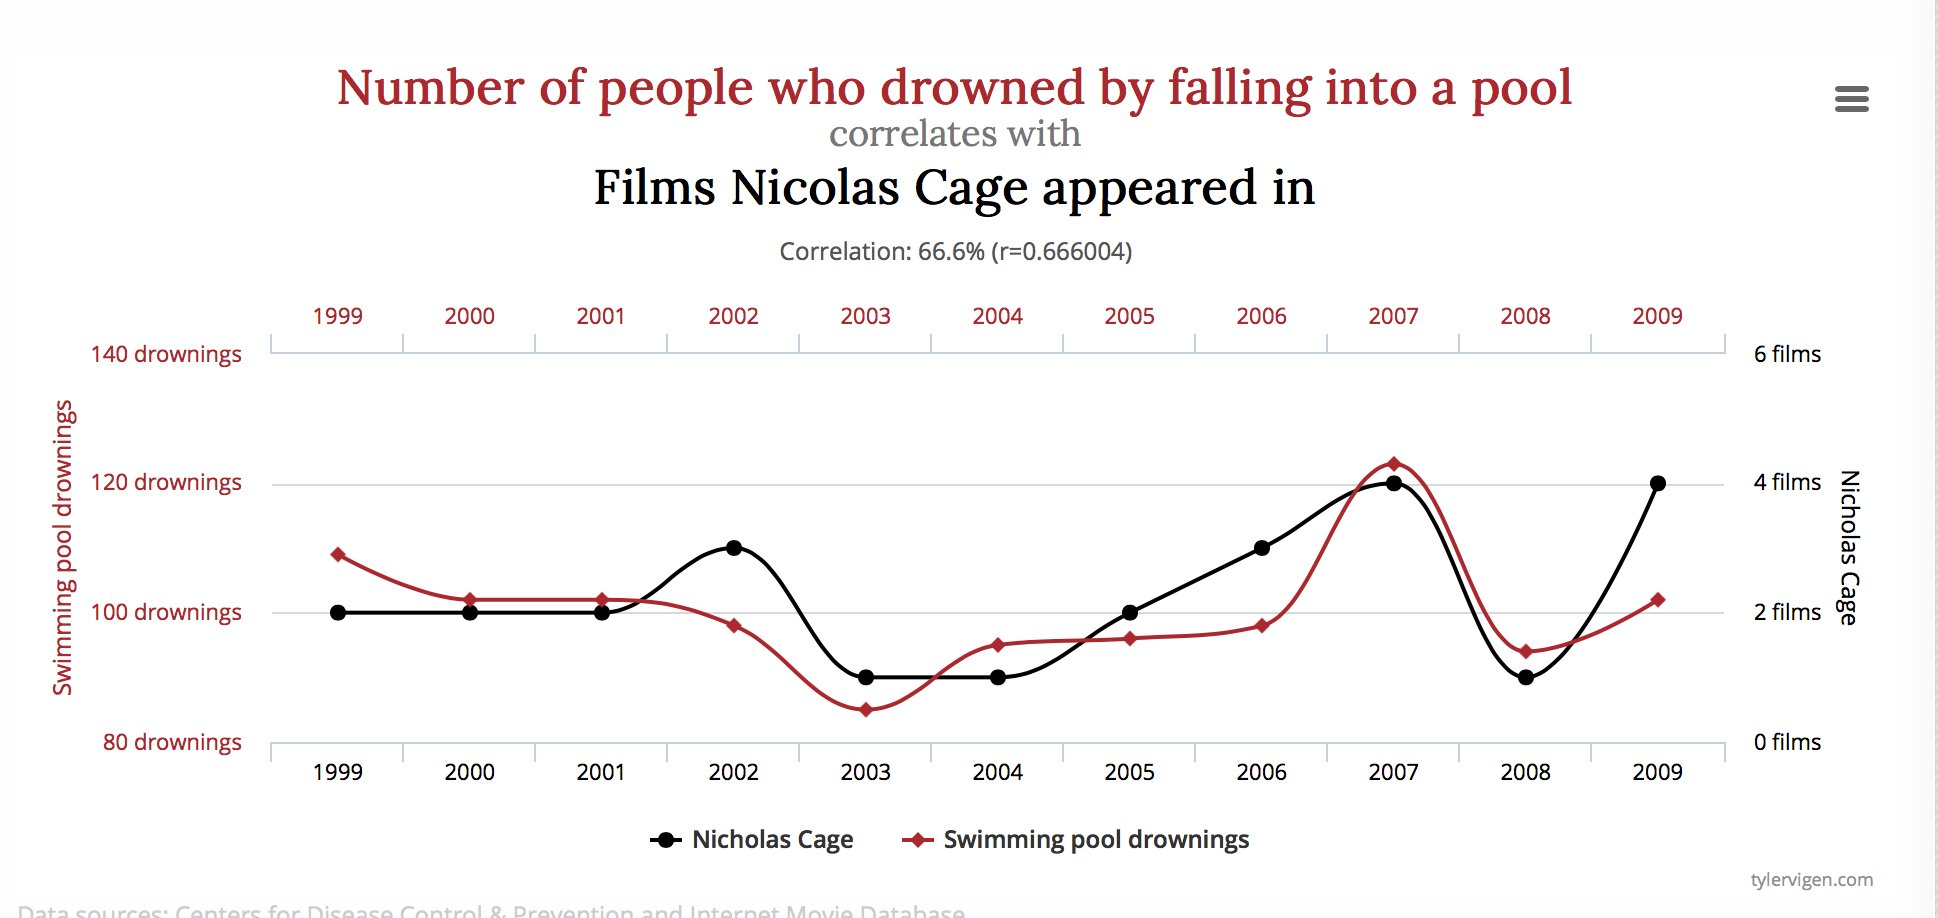
\includegraphics[width=0.8\linewidth,height=\textheight,keepaspectratio]{figs/corr_not_caus.jpeg}
\end{center}
\end{frame}

\begin{frame}{Correlation is not causation}
\protect\phantomsection\label{correlation-is-not-causation}
\begin{itemize}
\item
  When \(x\) is useful for predicting \(y\), it is not necessarily
  causing \(y\).
\item
  e.g., predict number of drownings \(y\) using number of ice-creams
  sold \(x\).
\item
  Correlations are useful for forecasting, even when there is no
  causality.
\item
  Better models usually involve causal relationships (e.g., temperature
  \(x\) and people \(z\) to predict drownings \(y\)).
\end{itemize}
\end{frame}

\begin{frame}{Multicollinearity}
\protect\phantomsection\label{multicollinearity}
In regression analysis, multicollinearity occurs when:

\begin{itemize}
\tightlist
\item
  Two predictors are highly correlated (i.e., the correlation between
  them is close to \(\pm1\)).
\item
  A linear combination of some of the predictors is highly correlated
  with another predictor.
\item
  A linear combination of one subset of predictors is highly correlated
  with a linear combination of another subset of predictors.
\end{itemize}
\end{frame}

\begin{frame}{Multicollinearity}
\protect\phantomsection\label{multicollinearity-1}
If multicollinearity exists\dots

\begin{itemize}
\tightlist
\item
  the numerical estimates of coefficients may be wrong (worse in Excel
  than in a statistics package)
\item
  don't rely on the \(p\)-values to determine significance.
\item
  there is no problem with model \emph{predictions} provided the
  predictors used for forecasting are within the range used for fitting.
\item
  omitting variables can help.
\item
  combining variables can help.
\end{itemize}
\end{frame}

\begin{frame}{Outliers and influential observations}
\protect\phantomsection\label{outliers-and-influential-observations}
\textbf{Things to watch for}

\begin{itemize}
\tightlist
\item
  \emph{Outliers}: observations that produce large residuals.
\item
  \emph{Influential observations}: removing them would markedly change
  the coefficients. (Often outliers in the \(x\) variable).
\item
  \emph{Lurking variable}: a predictor not included in the regression
  but which has an important effect on the response.
\item
  Points should not normally be removed without a good explanation of
  why they are different.
\end{itemize}
\end{frame}

\begin{frame}{Modern regression models}
\protect\phantomsection\label{modern-regression-models}
\begin{itemize}
\tightlist
\item
  Suppose instead of 3 regressors we had 44.

  \begin{itemize}
  \tightlist
  \item
    For example, 44 predictors leads to 18 trillion possible models!
  \end{itemize}
\item
  Stepwise regression cannot solve this problem due to the number of
  variables.
\item
  We need to use the family of Lasso models: lasso, ridge, elastic net
\end{itemize}
\end{frame}

\section{Some useful predictors for regression
models}\label{some-useful-predictors-for-regression-models}

\begin{frame}{Dummy variables}
\protect\phantomsection\label{dummy-variables}
\begin{textblock}{6}(0.4,1.5)
If a categorical variable takes only two values (e.g., `Yes'
or `No'), then an equivalent numerical variable can be constructed taking value 1 if yes and 0 if no. This is called a \textbf{dummy variable}.
\end{textblock}

\placefig{7.7}{1.}{width=5cm}{dummy2}
\end{frame}

\begin{frame}{Dummy variables}
\protect\phantomsection\label{dummy-variables-1}
\begin{textblock}{5}(0.4,1.5)
If there are more than two categories, then the variable can
be coded using several dummy variables (one fewer than the total number of categories).

\end{textblock}

\placefig{5.5}{1.5}{width=7.3cm}{dummy3}
\end{frame}

\begin{frame}{Beware of the dummy variable trap!}
\protect\phantomsection\label{beware-of-the-dummy-variable-trap}
\begin{itemize}
\item
  Using one dummy for each category gives too many dummy variables!
\item
  The regression will then be singular and inestimable.
\item
  Either omit the constant, or omit the dummy for one category.
\item
  The coefficients of the dummies are relative to the omitted category.
\end{itemize}
\end{frame}

\begin{frame}{Uses of dummy variables}
\protect\phantomsection\label{uses-of-dummy-variables}
\fontsize{13}{15}\sf

\textbf{Seasonal dummies}

\begin{itemize}
\tightlist
\item
  For quarterly data: use 3 dummies
\item
  For monthly data: use 11 dummies
\item
  For daily data: use 6 dummies
\end{itemize}

\pause

\textbf{Outliers}

\begin{itemize}
\tightlist
\item
  If there is an outlier, you can use a dummy variable to remove its
  effect.
\end{itemize}

\pause

\textbf{Public holidays}

\begin{itemize}
\tightlist
\item
  For daily data: if it is a public holiday, dummy=1, otherwise dummy=0.
\end{itemize}
\end{frame}

\begin{frame}[fragile]{Intervention variables}
\protect\phantomsection\label{intervention-variables}
\fontsize{12}{13}\sf

\textbf{Spikes}

\begin{itemize}
\tightlist
\item
  Equivalent to a dummy variable for handling an outlier. \pause
\end{itemize}

\textbf{Steps}

\begin{itemize}
\tightlist
\item
  Variable takes value 0 before the intervention and 1 afterwards.
  \pause
\end{itemize}

\textbf{Change of slope}

\begin{itemize}
\item
  Variables take values 0 before the intervention and values
  \(\{1,2,3,\dots\}\) afterwards.
\item
  this could be also handled using \texttt{trend()}
\end{itemize}
\end{frame}

\begin{frame}{Include special event using dummies}
\protect\phantomsection\label{include-special-event-using-dummies}
\begin{itemize}
\tightlist
\item
  Christmas Eve: if Christmas Eve, \(v_t=1\), \(v_t=0\) otherwise
\item
  New year's Day: if New year's Day, \(v_t=1\), \(v_t=0\) otherwise.
\item
  and more: Ramadan and Chinese new year, school holiday, etc
\end{itemize}
\end{frame}

\begin{frame}[fragile]{Interactions}
\protect\phantomsection\label{interactions}
For example, sometimes the effect of a particular event might be
different if it is on a weekend or a week day or its effect might be
different in each shift:

\begin{itemize}
\tightlist
\item
  you need to introduce an interaction variable
\item
  you can use a new dummy as : \texttt{v1*v2}
\end{itemize}
\end{frame}

\begin{frame}{Lagged predictors}
\protect\phantomsection\label{lagged-predictors}
The model include present and past values of predictor:
\(x_t,x_{t-1},x_{t-2},\dots.\)

\[
y_{t} = a + \beta_{0} x_{t} + \beta_{1} x_{t-1} + \dots + \beta_{k} x_{t-k} + \varepsilon_{t}
\]

\begin{itemize}
\tightlist
\item
  \(x\) can influence \(y\), but \(y\) is not allowed to influence
  \(x\).
\end{itemize}
\end{frame}

\begin{frame}{Lagged predictors}
\protect\phantomsection\label{lagged-predictors-1}
\begin{itemize}
\tightlist
\item
  Lagged values of a predictor:

  \begin{itemize}
  \tightlist
  \item
    Create new variables by shifting the existing variable backwards
  \end{itemize}
\end{itemize}

Example: \(x\) is advertising which has a delayed effect

\begin{align*}
  x_{1} &= \text{advertising for previous month;} \\
  x_{2} &= \text{advertising for two months previously;} \\
        & \vdots \\
  x_{m} &= \text{advertising for $m$ months previously.}
\end{align*}
\end{frame}

\begin{frame}[fragile]{Example: Insurance quotes and TV adverts}
\protect\phantomsection\label{example-insurance-quotes-and-tv-adverts}
\fontsize{12}{12}\sf

\begin{Shaded}
\begin{Highlighting}[]
\NormalTok{insurance}
\end{Highlighting}
\end{Shaded}

\begin{verbatim}
# A tsibble: 40 x 3 [1M]
      Month Quotes TVadverts
      <mth>  <dbl>     <dbl>
 1 2002 Jan   13.0      7.21
 2 2002 Feb   15.4      9.44
 3 2002 Mar   13.2      7.53
 4 2002 Apr   13.0      7.21
 5 2002 May   15.4      9.44
 6 2002 Jun   11.7      6.42
 7 2002 Jul   10.1      5.81
 8 2002 Aug   10.8      6.20
 9 2002 Sep   13.3      7.59
10 2002 Oct   14.6      8.00
# i 30 more rows
\end{verbatim}
\end{frame}

\begin{frame}{Example: Insurance quotes and TV adverts}
\protect\phantomsection\label{example-insurance-quotes-and-tv-adverts-1}
\pandocbounded{\includegraphics[keepaspectratio]{03_regression_files/figure-beamer/tvadvert-1.pdf}}
\end{frame}

\begin{frame}{Example: Insurance quotes and TV adverts}
\protect\phantomsection\label{example-insurance-quotes-and-tv-adverts-2}
\pandocbounded{\includegraphics[keepaspectratio]{03_regression_files/figure-beamer/tvadvertpairs-1.pdf}}
\end{frame}

\begin{frame}[fragile]{Example: Insurance quotes and TV adverts}
\protect\phantomsection\label{example-insurance-quotes-and-tv-adverts-3}
\fontsize{10}{10}\sf

\begin{Shaded}
\begin{Highlighting}[]
\NormalTok{fit }\OtherTok{\textless{}{-}}\NormalTok{ insurance }\SpecialCharTok{|\textgreater{}}
  \CommentTok{\# Restrict data so models use same fitting period}
  \FunctionTok{mutate}\NormalTok{(}\AttributeTok{Quotes =} \FunctionTok{c}\NormalTok{(}\ConstantTok{NA}\NormalTok{, }\ConstantTok{NA}\NormalTok{, }\ConstantTok{NA}\NormalTok{, Quotes[}\DecValTok{4}\SpecialCharTok{:}\DecValTok{40}\NormalTok{])) }\SpecialCharTok{|\textgreater{}}
  \FunctionTok{model}\NormalTok{(}
    \FunctionTok{ARIMA}\NormalTok{(Quotes }\SpecialCharTok{\textasciitilde{}} \FunctionTok{pdq}\NormalTok{(}\AttributeTok{d =} \DecValTok{0}\NormalTok{) }\SpecialCharTok{+}\NormalTok{ TVadverts),}
    \FunctionTok{ARIMA}\NormalTok{(Quotes }\SpecialCharTok{\textasciitilde{}} \FunctionTok{pdq}\NormalTok{(}\AttributeTok{d =} \DecValTok{0}\NormalTok{) }\SpecialCharTok{+}\NormalTok{ TVadverts }\SpecialCharTok{+}
      \FunctionTok{lag}\NormalTok{(TVadverts)),}
    \FunctionTok{ARIMA}\NormalTok{(Quotes }\SpecialCharTok{\textasciitilde{}} \FunctionTok{pdq}\NormalTok{(}\AttributeTok{d =} \DecValTok{0}\NormalTok{) }\SpecialCharTok{+}\NormalTok{ TVadverts }\SpecialCharTok{+}
      \FunctionTok{lag}\NormalTok{(TVadverts) }\SpecialCharTok{+}
      \FunctionTok{lag}\NormalTok{(TVadverts, }\DecValTok{2}\NormalTok{)),}
    \FunctionTok{ARIMA}\NormalTok{(Quotes }\SpecialCharTok{\textasciitilde{}} \FunctionTok{pdq}\NormalTok{(}\AttributeTok{d =} \DecValTok{0}\NormalTok{) }\SpecialCharTok{+}\NormalTok{ TVadverts }\SpecialCharTok{+}
      \FunctionTok{lag}\NormalTok{(TVadverts) }\SpecialCharTok{+}
      \FunctionTok{lag}\NormalTok{(TVadverts, }\DecValTok{2}\NormalTok{) }\SpecialCharTok{+}
      \FunctionTok{lag}\NormalTok{(TVadverts, }\DecValTok{3}\NormalTok{))}
\NormalTok{  )}
\end{Highlighting}
\end{Shaded}
\end{frame}

\begin{frame}[fragile]{Example: Insurance quotes and TV adverts}
\protect\phantomsection\label{example-insurance-quotes-and-tv-adverts-4}
\fontsize{10}{10}\sf

\begin{Shaded}
\begin{Highlighting}[]
\FunctionTok{glance}\NormalTok{(fit)}
\end{Highlighting}
\end{Shaded}

{\def\LTcaptype{none} % do not increment counter
\begin{longtable}[]{@{}rrrrrr@{}}
\toprule\noalign{}
Lag order & sigma2 & log\_lik & AIC & AICc & BIC \\
\midrule\noalign{}
\endhead
0 & 0.265 & -28.3 & 66.6 & 68.3 & 75.0 \\
1 & 0.209 & -24.0 & 58.1 & 59.9 & 66.5 \\
2 & 0.215 & -24.0 & 60.0 & 62.6 & 70.2 \\
3 & 0.206 & -22.2 & 60.3 & 65.0 & 73.8 \\
\bottomrule\noalign{}
\end{longtable}
}
\end{frame}

\begin{frame}[fragile]{Example: Insurance quotes and TV adverts}
\protect\phantomsection\label{example-insurance-quotes-and-tv-adverts-5}
\fontsize{8}{9}\sf

\begin{Shaded}
\begin{Highlighting}[]
\CommentTok{\# Re{-}fit to all data}
\NormalTok{fit }\OtherTok{\textless{}{-}}\NormalTok{ insurance }\SpecialCharTok{|\textgreater{}}
  \FunctionTok{model}\NormalTok{(}\FunctionTok{ARIMA}\NormalTok{(Quotes }\SpecialCharTok{\textasciitilde{}}\NormalTok{ TVadverts }\SpecialCharTok{+} \FunctionTok{lag}\NormalTok{(TVadverts) }\SpecialCharTok{+} \FunctionTok{pdq}\NormalTok{(}\AttributeTok{d =} \DecValTok{0}\NormalTok{)))}
\FunctionTok{report}\NormalTok{(fit)}
\end{Highlighting}
\end{Shaded}

\begin{verbatim}
Series: Quotes 
Model: LM w/ ARIMA(1,0,2) errors 

Coefficients:
        ar1    ma1    ma2  TVadverts  lag(TVadverts)  intercept
      0.512  0.917  0.459     1.2527          0.1464       2.16
s.e.  0.185  0.205  0.190     0.0588          0.0531       0.86

sigma^2 estimated as 0.2166:  log likelihood=-23.9
AIC=61.9   AICc=65.4   BIC=73.7
\end{verbatim}

\pause

\begin{block}{}
\protect\phantomsection\label{section}
\fontsize{13}{13}\sf\vspace*{-0.7cm}\begin{align*}
  y_t &= 2.16 +
         1.25 x_t +
         0.15 x_{t-1} + \eta_t,\\
  \eta_t &= 0.512 \eta_{t-1} +
        \varepsilon_t +
        0.92 \varepsilon_{t-1} +
        0.46 \varepsilon_{t-2}.
\end{align*}
\end{block}
\end{frame}

\begin{frame}[fragile]{Example: Insurance quotes and TV adverts}
\protect\phantomsection\label{example-insurance-quotes-and-tv-adverts-6}
\fontsize{11}{13}\sf

\begin{Shaded}
\begin{Highlighting}[]
\NormalTok{advert\_a }\OtherTok{\textless{}{-}} \FunctionTok{new\_data}\NormalTok{(insurance, }\DecValTok{20}\NormalTok{) }\SpecialCharTok{|\textgreater{}}
  \FunctionTok{mutate}\NormalTok{(}\AttributeTok{TVadverts =} \DecValTok{10}\NormalTok{)}
\FunctionTok{forecast}\NormalTok{(fit, advert\_a) }\SpecialCharTok{|\textgreater{}} \FunctionTok{autoplot}\NormalTok{(insurance)}
\end{Highlighting}
\end{Shaded}

\pandocbounded{\includegraphics[keepaspectratio]{03_regression_files/figure-beamer/unnamed-chunk-8-1.pdf}}
\end{frame}

\begin{frame}[fragile]{Example: Insurance quotes and TV adverts}
\protect\phantomsection\label{example-insurance-quotes-and-tv-adverts-7}
\fontsize{11}{13}\sf

\begin{Shaded}
\begin{Highlighting}[]
\NormalTok{advert\_b }\OtherTok{\textless{}{-}} \FunctionTok{new\_data}\NormalTok{(insurance, }\DecValTok{20}\NormalTok{) }\SpecialCharTok{|\textgreater{}}
  \FunctionTok{mutate}\NormalTok{(}\AttributeTok{TVadverts =} \DecValTok{8}\NormalTok{)}
\FunctionTok{forecast}\NormalTok{(fit, advert\_b) }\SpecialCharTok{|\textgreater{}} \FunctionTok{autoplot}\NormalTok{(insurance)}
\end{Highlighting}
\end{Shaded}

\pandocbounded{\includegraphics[keepaspectratio]{03_regression_files/figure-beamer/unnamed-chunk-9-1.pdf}}
\end{frame}

\begin{frame}[fragile]{Example: Insurance quotes and TV adverts}
\protect\phantomsection\label{example-insurance-quotes-and-tv-adverts-8}
\fontsize{11}{13}\sf

\begin{Shaded}
\begin{Highlighting}[]
\NormalTok{advert\_c }\OtherTok{\textless{}{-}} \FunctionTok{new\_data}\NormalTok{(insurance, }\DecValTok{20}\NormalTok{) }\SpecialCharTok{|\textgreater{}}
  \FunctionTok{mutate}\NormalTok{(}\AttributeTok{TVadverts =} \DecValTok{6}\NormalTok{)}
\FunctionTok{forecast}\NormalTok{(fit, advert\_c) }\SpecialCharTok{|\textgreater{}} \FunctionTok{autoplot}\NormalTok{(insurance)}
\end{Highlighting}
\end{Shaded}

\pandocbounded{\includegraphics[keepaspectratio]{03_regression_files/figure-beamer/unnamed-chunk-10-1.pdf}}
\end{frame}

\begin{frame}{Lead predictors}
\protect\phantomsection\label{lead-predictors}
Sometimes a change in the predictor \(x_t\) that will happen in the
future will affect the value of \(y_t\) in the past. We say \(x_t\) is a
leading indicator.

\begin{itemize}
\tightlist
\item
  Lead values of a predictor:

  \begin{itemize}
  \tightlist
  \item
    Create new variables by shifting the existing variable forwards
  \end{itemize}
\end{itemize}

\begin{block}{}
\begin{itemize}
  \item $y_t=$ sales, $x_t=$ tax policy announcement
\end{itemize}
\end{block}
\end{frame}




\end{document}
